\documentclass[a4paper, 12pt]{article}
\usepackage{graphicx}
\graphicspath{{images/}}
\usepackage{listings}
\usepackage[english]{babel}
\usepackage{caption}
\usepackage{color}

\title{Homework 1}
\author{Nasir Mohammad Khalid}
\date{March 9, 2019}

\makeatletter
\let\thetitle\@title
\let\theauthor\@author
\let\thedate\@date
\makeatother

\definecolor{codegreen}{rgb}{0,0.6,0}
\definecolor{codegray}{rgb}{0.5,0.5,0.5}
\definecolor{codepurple}{rgb}{0.58,0,0.82}
\definecolor{backcolour}{rgb}{0.95,0.95,0.92}

\lstdefinestyle{mystyle}{
    backgroundcolor=\color{backcolour},   
    commentstyle=\color{codegreen},
    keywordstyle=\color{magenta},
    numberstyle=\tiny\color{codegray},
    stringstyle=\color{codepurple},
    basicstyle=\scriptsize,
    breakatwhitespace=false,         
    breaklines=true,                 
    captionpos=b,                    
    keepspaces=true,                 
    numbers=left,                    
    numbersep=1pt,                  
    showspaces=false,                
    showstringspaces=false,
    showtabs=false,                  
    tabsize=1
}
 
\lstset{style=mystyle}

\begin{document} 
    \begin{titlepage}
        \centering
        \vspace*{0.5 cm}
        
\includegraphics[scale = 0.60]{logo.png}\\[1.0 cm]	% University Logo
        \textsc{\LARGE American University of Sharjah}\\[1.0 cm]
        \textsc{\Large ELE494-09}\\[0.2 cm]	
        \textsc{\Large Deep Networks in Machine Learning}\\[0.5 cm]			% Course Code
        \rule{\linewidth}{0.2 mm} \\[0.4 cm]
        { \huge \bfseries \thetitle}\\
        \rule{\linewidth}{0.2 mm} \\[1.5 cm]
        
        \textsc{\Large{\theauthor}}\\[0.3 cm]
        \textsc{\Large{65082}}\\[0.3 cm]
        \textsc{\Large{\thedate}}\\[1.5 cm]

        \textmd{Submitted To: \itshape{Dr.Usman Tariq}}
    \end{titlepage}

    \clearpage
    \tableofcontents
    \listoffigures
    \lstlistoflistings
    \clearpage

    \section{Theoretical}

    \subsection{Q1}

    \textbf{For a 3 dimensional dataset, What is the minimum number of points that are required to fit a hyperplane?}\\
    
    For a 3 dimensional dataset we would have: 

    $$y = w_0 + [w_1 w_2 w_3] * [x_1 x_2 x_3]^T$$

    Therefore the hyperplane is a 2D plane which requires a minimum of 3 points. 

    \subsection{Q2}

    \textbf{Write a summary on the paper 'Deep Learning'}\\

    The paper begins by explaining how recent advances in deep learning have allowed machines to teach them selves to identify patterns in high dimensional data. It then discusses supervised learning and explains how a basic neural net works using an error function and then trying to minimize output by using the stochastic gradient descent. The paper explains how this technique only works on shallow data and feature extractors are needed to make it applicable to more complex data as well as invariant to . Before discussing the use of these feature extractors the paper first explains the principle of backpropogation and also discusses briefly that the issue of wrong minima in gradient descent is not a major one. After this it discusses the convolutional neural networks and how they are used to process data that is in the form of multiple arrays. They use pooling and convolution along with certain filter banks, the success of these feedforward networks have made them the standard for image related learning. A network that uses CNN + RNN is discussed which is able to identify objects and features of images using the CNN and after this the RNN creates a caption for the image. The paper then discusses how hidden layers of the network learn to represent the data as a sequential decomposition in to simpler forms, due to these distributed representations the networks are great at prediction and one such example discussed is how computers can predict what a person will type next. The second last section is about the Recurrent neural networks and how they are great for predictive behaviour and their main objective is to learn about long-term dependencies. The final section discusses the future of deep learning and how the authours believe that the way forward for innovation is in unsupervised learning.

    \subsection{Q3}

    \textbf{What is the difference between deep and shallow learning. Explain with concrete example(s) when shallow learning is suitable as compared to deep learning and vise versa. }\\

    Shallow learning cases are those where data can be easily segregated in to different classes and the entire network is made up of a single hidden layer containing few neurons. In these cases the dataset provided is already labelled and the computer simply learns how to fit the data with it's labels. Often this is just a binary classification problem.\\

    In deep learning however we provide the network with some data and expect it to identify the patterns and classify the output on its own. This sort of learning often consists of a huge number of hidden layers each consisting of a large number of neurons.\\

    Examples of shallow learning often include linear regression or binary classification problems where the data can be easily split without the need of higher level transformations. One example is guessing the price of a house based on it's square feet. Here we would use previous data of area vs price and linear regression to get a price for given area. It is useful when space can be carved in to half-spaces separated by a hyperplane.\\

    Examples of deep learning are in cases where we have just input data and are looking for our network to learn and find patterns. One example is face recognition or even identifying different breeds of dogs because in both these cases a much higher order transformation is needed to sufficiently identify patterns.\\

    \pagebreak

    \section{Implementation}

    \subsection{Cost function and Gradient Descent}

    Here we take the error function to be the mean squared error give as:

    $$Error = \frac{1}{N} * \sum_{n \in data} (t_n - y_n)^2 $$

    The derivative of this function with respect to the weights is given by (epsilon includes extra terms from taking derivative):

    $$\Delta w = \frac{1}{N} * \sum_{n \in data} \epsilon * x_n * (t_n - y_n) $$

    In this case we have only one weight since we are using a linear neuron so it becomes:

    $$\Delta w = \epsilon * x_n * (t_n - y_n) $$

    We also have one bias and the input for it is one so $ x_n = 1 $ therefore it simplifies to:

    $$\Delta b = \epsilon * 1 * (t_n - y_n) $$

    \subsection{Defining Neurons and Initial Code [Cell 1]}

    \begin{lstlisting}[language=python, caption=Initialization Code (Cell 1)]
    # Importing all required libraries
    import numpy as np
    import matplotlib.pyplot as plt
    import pickle as pkl

    # Importing all required datasets
    (x_train_1, y_train_1), (x_test_1, y_test_1) = pkl.load( open( "dataset.pkl", "rb" ) )
    (x_train_2, y_train_2), (x_test_2, y_test_2)= pkl.load( open( "dataset2.pkl", "rb" ) )

    # Making sure all loaded data is a 1D Tensor
    x_train_1 = x_train_1.flatten()
    y_train_1 = y_train_1.flatten()
    x_test_1 = x_test_1.flatten()
    y_test_1 = y_test_1.flatten()
    x_train_2 = x_train_2.flatten()
    y_train_2 = y_train_2.flatten()
    x_test_2 = x_test_2.flatten()
    y_test_2 = y_test_2.flatten()


    # Defining a neuron class
    class neuron:
        def __init__(self, weight, bias):
            self.weight = weight
            self.bias = bias
        
        def fire(self, x):
            self.output = (self.weight * x) + self.bias
            return self.output
        
        def error(self, y_actual):
            self.err = self.output - y_actual
            return self.err
        
        def mse(self, y_actual):
            return (1/len(y_actual) * ((y_actual - self.output)*(y_actual - self.output)).sum())
            
        def grad_des(self, x, rate):
            for i, val in enumerate(x):
                self.weight -= val * self.err[i] * rate
                self.bias -= self.err[i] * rate
            
        def plot(self, x, y, title):
            plt.plot(x, y, 'ro', x, self.output)
            plt.title(title)
            plt.show(block=False)
            

    # Creating a neuron for the first dataset with initialized weight = bias = 1
    N1 = neuron(1, 1)

    # Creating a neuron for the second dataset with initialized weight = bias = 1
    N2 = neuron(1, 1)

    # Learning rate for the first neuron (dataset_1)
    lr_1 = 0.00001

    # Learning rate for the first neuron (dataset_2)
    lr_2 = 0.001

    # Learning rates were decided after a lot of trial and error. Dataset 1 tends
    # to oscillate and eventually 'explode' for a larger learning rate than the one used.\end{lstlisting}

    \pagebreak

    \subsection{Training Neuron 1 for Dataset 1 [Cell 2]}

    \begin{lstlisting}[language=python, caption=Dataset 1 Training Code (Cell 2)]
    # Here we train N1 for dataset 1

    loops = 20000
    print("Training N1 for Dataset 1")
    print("--------------------------------------------")
    for z in range(0, loops + 1):
        # Activate the first neuron and get an output
        N1.fire(x_train_1)
        
        # Get the first error based on the previous output
        error_N1 = N1.error(y_train_1)
    
        # Perform gradient descent using input with learning rate of lr_1
        N1.grad_des(x_train_1, lr_1)
    
        if (z%(loops/10)) == 0:
            N1.plot(x_train_1, y_train_1, 'N1 (dataset 1) at iteration ' + str(z))
            print("Error on iteration " + str(z) + " = " + str(error_N1.sum()))
            print("MSE Error on iteration " + str(z) + " = " + str(N1.mse(y_train_1)))
            print("Weight on iteration " + str(z) + " = " + str(N1.weight))
            print("Bias on iteration " + str(z) + " = " + str(N1.bias) + '\n')
            
    
    print("--------------------------------------------")\end{lstlisting}

    \begin{figure}[h!]
        \centering
        \captionsetup{justification=centering}
        \centering
            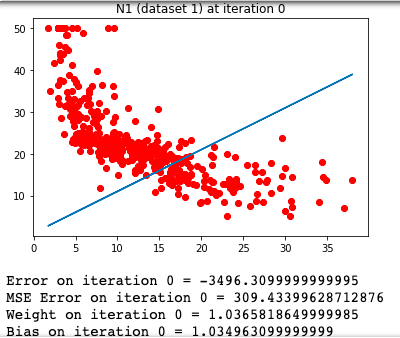
\includegraphics[width=0.6\textwidth]{1.png}
            \caption{Data anad Neuron on 0th Iteration}
    \end{figure}

    \begin{figure}[h!]
        \centering
        \captionsetup{justification=centering}
        \centering
            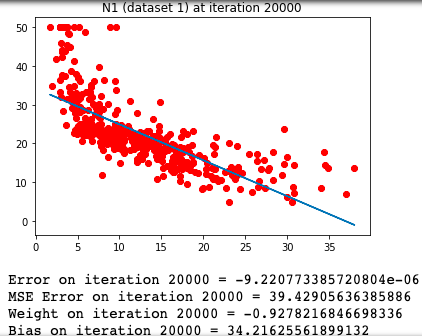
\includegraphics[width=0.6\textwidth]{2.png}
            \caption{Data anad Neuron on 20000th Iteration}
    \end{figure}

    \pagebreak

    \subsection{Testing Neuron 1 with Test Data [Cell 3]}

    \begin{lstlisting}[language=python, caption=Dataset 1 Testing Code (Cell 3)]
    # FOR N1: Here we get the final weight and bias. Then we test on the test data

    # Fire neuron for test input
    N1.fire(x_test_1)
    
    # Getting the mean squared error 
    error = N1.mse(y_test_1)
    
    # Plot test data and the Neuron line
    plt.plot(x_test_1, y_test_1, 'ro', x_test_1, N1.fire(x_test_1))
    plt.title('Test data and the N1 Neuron')
    plt.show(block=False)
    
    print("Final weight = " + str(N1.weight))
    print("Final bias = " + str(N1.bias))
    print("The MSE error for test data = " + str(error))\end{lstlisting}
        
    \begin{figure}[h!]
        \centering
        \captionsetup{justification=centering}
        \centering
            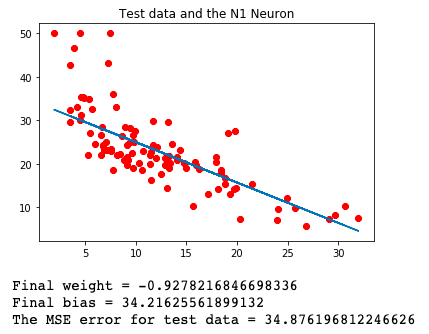
\includegraphics[width=0.6\textwidth]{3.png}
            \caption{Test Data 1 and Neuron}
    \end{figure}

    \pagebreak

    \subsection{Training Neuron 2 for Dataset 2 [Cell 4]}

    \begin{lstlisting}[language=python, caption=Dataset 2 Training Code (Cell 2)]
    # Here we train N2 for dataset 2

    loops = 20000
    print("Training N2 for Dataset 2")
    print("--------------------------------------------")
    for z in range(0, loops + 1):
        # Activate the first neuron and get an output
        N2.fire(x_train_2)
        
        # Get the first error based on the previous output
        error_N2 = N2.error(y_train_2)
    
        # Perform gradient descent using input with learning rate of lr_2
        N2.grad_des(x_train_2, lr_2)
    
        if (z%(loops/10)) == 0:
            N2.plot(x_train_2, y_train_2, 'N2 (dataset 2) at iteration ' + str(z))
            print("Error on iteration " + str(z) + " = " + str(error_N2.sum()))
            print("MSE Error on iteration " + str(z) + " = " + str(N2.mse(y_train_1)))
            print("Weight on iteration " + str(z) + " = " + str(N2.weight))
            print("Bias on iteration " + str(z) + " = " + str(N2.bias) + '\n')
            
    
    print("--------------------------------------------")\end{lstlisting}

    \begin{figure}[h!]
        \centering
        \captionsetup{justification=centering}
        \centering
            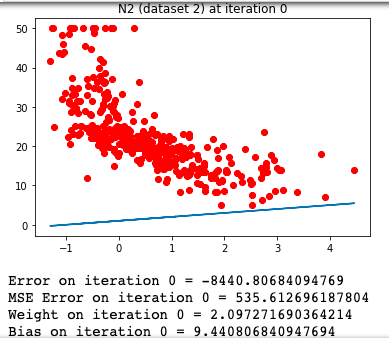
\includegraphics[width=0.6\textwidth]{4.png}
            \caption{Data anad Neuron on 0th Iteration}
    \end{figure}

    \begin{figure}[h!]
        \centering
        \captionsetup{justification=centering}
        \centering
            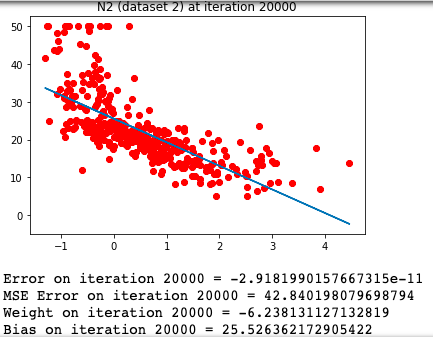
\includegraphics[width=0.6\textwidth]{5.png}
            \caption{Data anad Neuron on 20000th Iteration}
    \end{figure}

    \pagebreak

    \subsection{Testing Neuron 2 with Test Data [Cell 5]}

    \begin{lstlisting}[language=python, caption=Dataset 2 Testing Code (Cell 5)]
    # FOR N2: Here we get the final weight and bias. Then we test on the test data

    # Fire neuron for test input
    N2.fire(x_test_2)

    # Getting the mean squared error 
    error = N2.mse(y_test_2)

    # Plot test data and the Neuron line
    plt.plot(x_test_2, y_test_2, 'ro', x_test_2, N2.fire(x_test_2))
    plt.title('Test data and the N2 Neuron')
    plt.show(block=False)

    print("Final weight = " + str(N2.weight))
    print("Final bias = " + str(N2.bias))
    print("The MSE error for test data = " + str(error))\end{lstlisting}

    \begin{figure}[h!]
        \centering
        \captionsetup{justification=centering}
        \centering
            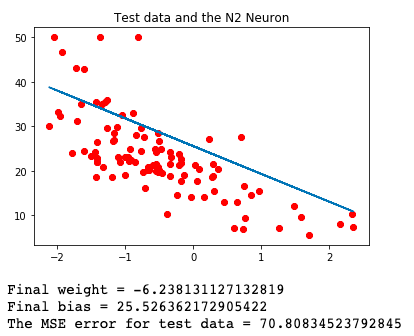
\includegraphics[width=0.6\textwidth]{6.png}
            \caption{Test Data 2 and Neuron}
    \end{figure}


    \subsection{Final Results for Test Data 1 and Neuron 1}

    $$Weight = -0.9278216846698336$$

    $$Bias = 34.21625561899132$$

    $$MSE\ error\ on\ Training\ Dataset\ = 39.42905636385886$$

    $$MSE\ error\ on\ Test\ Dataset\ = 34.876196812246626$$

    \subsection{Final Results for Test Data 2 and Neuron 2}

    $$Weight = -6.238131127132819$$

    $$Bias = 25.526362172905422$$

    $$MSE\ error\ on\ Training\ Dataset\ = 42.840198079698794$$

    $$MSE\ error\ on\ Test\ Dataset\ = 70.80834523792845$$
\end{document}